\documentclass[11pt, letterpaper]{article}

% Importing packages
\usepackage[left=0.75in, right=0.75in, top=1in, bottom=1in]{geometry}
\usepackage{amsmath}
\usepackage{xcolor}
\usepackage{graphicx}
\usepackage{caption}
\usepackage{subcaption}
\usepackage{tikz}
\usepackage{algorithm}% http://ctan.org/pkg/algorithms
\usepackage{algpseudocode}% http://ctan.org/pkg/algorithmicx
\usepackage{pdfpages}
\usepackage{hyperref}

\newcommand{\nameA}{Nikhil Sethukumar}
\newcommand{\nameB}{Vishnu Varadan}
\newcommand{\emailA}{nsethukumar@ethz.ch}
\newcommand{\emailB}{vvaradan@ethz.ch}
\newcommand{\rollA}{21-954-029}
\newcommand{\rollB}{21-957-725}
\newcommand{\projtitle}{Overcoming Braess's Paradox: A Modelling based Approach}

\title{\projtitle}
\author{\nameA, \nameB}
\hypersetup{
    unicode=true,
    pdftoolbar=false,
    pdfmenubar=false,
    pdffitwindow=false,
    pdftitle={\projtitle},
    pdfauthor={\nameA, \nameB},
    colorlinks=true,
    linkcolor=blue,
    citecolor=magenta,
    urlcolor=cyan
}

\newcommand{\bp}{Braess's paradox}
\newcommand{\NE}{Nash Equilibrium}

\newcommand{\nodeA}{\textcolor{blue}{A}}
\newcommand{\nodeB}{\textcolor{orange!80!black}{B}}
\newcommand{\nodeC}{\textcolor{orange!80!black}{C}}
\newcommand{\nodeD}{\textcolor{green!70!black}{D}}
\newcommand{\pathferry}{\textcolor{cyan!40!blue}{\textsf{ferry}}}
\newcommand{\pathalley}{\textcolor{red!40!brown}{\textsf{alley}}}
\newcommand{\pathbridge}{\textsf{bridge}}

\DeclareMathOperator*{\argmin}{argmin}
\newcommand{\bpdiag}[3]{
\begin{tikzpicture}
    \node (A) at (0,0) [thick, blue, circle, fill=blue!20] {A};
    \node (D) at (6,0) [thick, green!70!black, circle, fill=green!20] {D};
    \node (B) at (3,2) [thick, orange!80!black, circle, fill=orange!20] {B};
    \node (C) at (3,-2) [thick, orange!80!black, circle, fill=orange!20] {C};

    % ferry
    \draw [->, ultra thick, cyan!40!blue] (A)--(B) node[midway, anchor=south east]{$#1$};
    \draw [->, ultra thick, cyan!40!blue] (C)--(D) node[midway, anchor=north west]{$#1$};

    % alley
    \draw [->, ultra thick, red!40!brown] (A)--(C) node[midway, anchor=north east]{$#2+#3 n_{AC}$};
    \draw [->, ultra thick, red!40!brown] (B)--(D) node[midway, anchor=south west]{$#2+#3 n_{BD}$};

    % bridge
    \draw [<->, dotted, ultra thick] (B)--(C) node[midway,right]{0};

    % legend
    \draw [->, ultra thick, red!40!brown] (0.5,-3)--(1.5,-3) node[midway, anchor = north]{\textsf{alley}};
    \draw [<->, dotted, ultra thick] (2.5,-3)--(3.5,-3) node[midway, anchor = north]{\textsf{bridge}};
    \draw [->, ultra thick, cyan!40!blue] (4.5,-3)--(5.5,-3) node[midway, anchor = north]{\textsf{ferry}};
\end{tikzpicture}
}

\newcommand{\DAarch}[4]{
        \begin{tikzpicture}
        \def \n {20}
        \def \N {8}
        \def \radius {2cm}
        \def \rd {1mm}
        \def \rer {4mm}
        
        \def \margin {8} % margin in angles, depends on the radius
        
        \node[draw, circle] at (360:0mm) (ustar) {$a_{#1}$};
        \foreach \i [count=\ni from 0] in {#2,#3,#4}{
          \node[draw, circle] at ({108-\ni*40}:\radius) (u\ni) {$a_{\i}$};
          \node at ({115-\ni*40}:\radius/2) {};
          \draw[<-] (ustar)--(u\ni);
        }
        
        \draw[dotted,black] (15:\radius/2) arc[start angle=15, end angle=-250, radius=\radius/2]
        node[midway,below]{$\mathcal{N}_{#1}$};
        \end{tikzpicture}
}

\begin{document}
    
\includegraphics[width=2in]{ETHlogo.pdf}

\vspace{\stretch{2}}

\begin{center}

\Large \textsf{Complex Social Systems: Modeling Agents, Learning, and Games}

\textsf{Fall 2022}

\vspace{\stretch{1}}

\normalsize Project Report

\vspace{\stretch{2}}

\textbf{\huge{\projtitle}}

\vspace{\stretch{2}}

\Large{ \nameA, \nameB}

\vspace{\stretch{6}}

\large{
Zurich

\today}

\normalsize

\end{center}
\thispagestyle{empty}

\newpage

    \section*{Agreement for free-download}
    
    \large We hereby agree to make our source code for this project freely available for download from the web pages of the SOMS chair. Furthermore, we assure that all source code is written by ourselves and is not violating any copyright restrictions.

    \vfill

    \hspace*{\stretch{1}} \nameA \hspace*{\stretch{1}} \nameB \hspace*{\stretch{1}}

    
    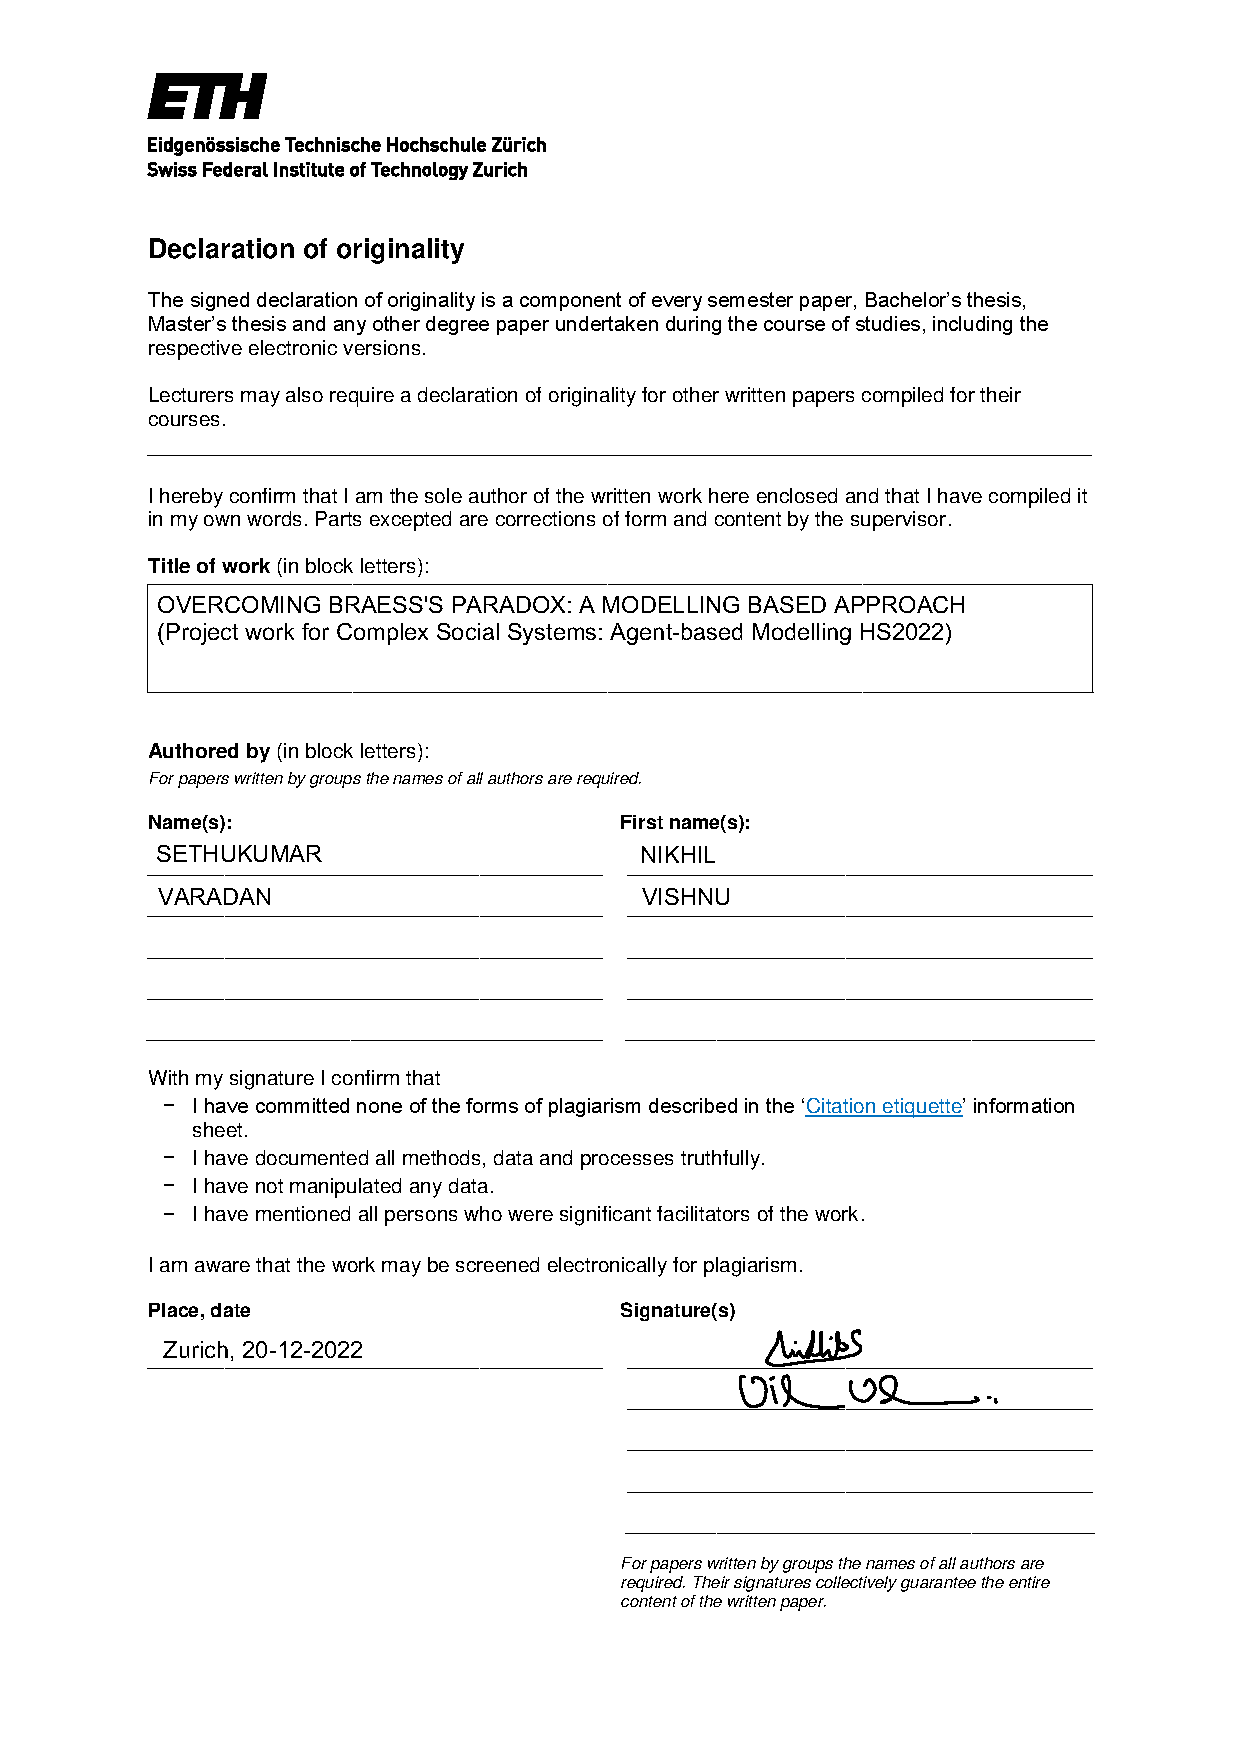
\includepdf{declaration-originality-signed.pdf}
   

    
\tableofcontents

\newpage


\section{Abstract}
The selection of route in a congestion game depends mainly on the density of traffic over the available routes. Selfish route choice does not always result in a lower time taken for an agent to get from the source to the destination when compared to strategies that are formed by cooperation by agents. Moreover, extension of the road network to redistribute the traffic flow can result in higher travel times for the agents leading to a paradoxical situation. In this work we investigate if an agent can be modelled such that the paradoxical effect can be mitigated in a distributed way with minimal coordination between the agents. 


\section{Individual contributions}
Nikhil was responsible for designing the Game, code the models in an object oriented manner in Python, for the Presentation and Report. He was also responsible for maintaining the repository on GitHub.

Vishnu came up with the models to mitigate the effect of the paradox. He also wrote MATLAB Code and performed Data Collection and was also responsible for the Presentation and the Report. 

\section{Introduction and Motivations}

\subsection{Mathematical Preliminaries of Game Theory}

Game theory provides a mathematical model for studying interactions between agents with a selfish interest \cite{hespanha}. We consider $i = 1 \ldots n$ \emph{agents} interacting, each with an \emph{action} $a_i \in \mathcal{A}_i$. The \emph{cost} incurred by agent $i$ is $J_i(a_1 \ldots a_n)$, which is what they try to minimize. This may be extended to multi-stage games by assuming action sets particular to a stage for each agent, and costs that can vary with the stage.

The game is said to be in a \emph{\NE}~when the set of actions of all agents $\{a_1^*, \ldots a_n^*\}$ are such that no one can unilaterally reduce their cost by changing their action. In other words, Equation~\eqref{eqn:NEcondition} is satisfied.

\begin{equation}
    \label{eqn:NEcondition}
    \text{for each agent}\ i,\quad a_i^* = \argmin_{a_i}\ J_i(a_i, a_{-i})
\end{equation}

where $a_{-i}$ represents the actions of the other agents $\{a_i \ldots a_{i-1}, a_{i+1} \ldots a_n\}$.

\emph{Social cost} is a number that indicates the welfare of all the agents. It could, for example, be the sum of costs of all agents. The \emph{price of anarchy} indicates how worse off the \NE~is as compared to the case with the least social cost ($\{a_1', \ldots a_n'\}$). They can, for example be defined as in Equation~\eqref{eqn:PoA}.

\begin{equation}
    \label{eqn:PoA}
    \text{Social Cost}\ = \sum_{i=1}^{n} J_i(a_i, a_{-i}) \quad \text{and}\quad \text{PoA} = \frac{\sum_{i=1}^{n} J_i(a_i^*, a_{-i}^*)}{\sum_{i=1}^{n} J_i(a_i', a_{-i}')}
\end{equation}

\subsection{\bp}

Congestion games are a special class of games in Game Theory, where the cost for each agent depends on the resources it chooses, which in turn varies with the number of agents choosing that resource. Traffic flow can be modelled as a congestion game where agents have to get from a start node to an end node. They can choose to pass through one of two intermediate nodes, with one leg of each path having travel time proportional to the number of agents using the leg. In this scenario, for specific choices of travel time over each connection, adding a connection of 0 travel time between the intermediate nodes can increase the \NE~travel time. This is called \bp~\cite{braess}.

\subsection{Relevance of \bp~and Previous Works}
\bp~is a counter-intuitive result and has occurred in real-life. One such instance is mentioned in a newspaper:

``ON Earth Day this year, New York City's Transportation Commissioner decided to close 42d Street, which as every New Yorker knows is always congested. \ldots 
But to everyone's surprise, Earth Day generated no historic traffic jam. Traffic flow actually improved when 42d Street was closed.

To mathematicians, this may be a real-world example of Braess's paradox, a statistical theorem that holds that when a network of streets is already jammed with vehicles, adding a new street can make traffic flow even more slowly.''\cite{nytimes} 

In a more theoretical aspect, the papers  \cite{braessexistence} and \cite{PAS1997265} explore the conditions in which the paradoxical situation might arise. Previous works have outlined the negatives of selfish routing and highlighted the importance of cooperative behaviour among the agents \cite{selfishrouting}. The work carried out in \cite{helbing2005individuals} especially focuses on the emergence of cooperation between agents in the selection of routes in a repeated game setup. The paper \cite{milinski2002reputation} introduces a currency like mechanism called as ``reputation" to overcome a similar problem that arises in a multistage tragedy of commons game setup.

\section{Description of the Model}

\subsection{Problem setup}
Let us begin with the basic problem formulation and then choose numbers that satisfy our conditions. Let us consider the case of crossing the Grand Canal in Venice. Let us assume that the Canal has dried up a bit beneath the Rialto and people who want to cross it would have to either take a ferry before the Rialto and then walk via an alley, or walk via an alley and then take a ferry after the Rialto, or walk via alleys on both banks and take the Rialto to cross the Canal. This is illustrated in Figure~\ref{fig:veniceill}.

\begin{figure}
    \centering
    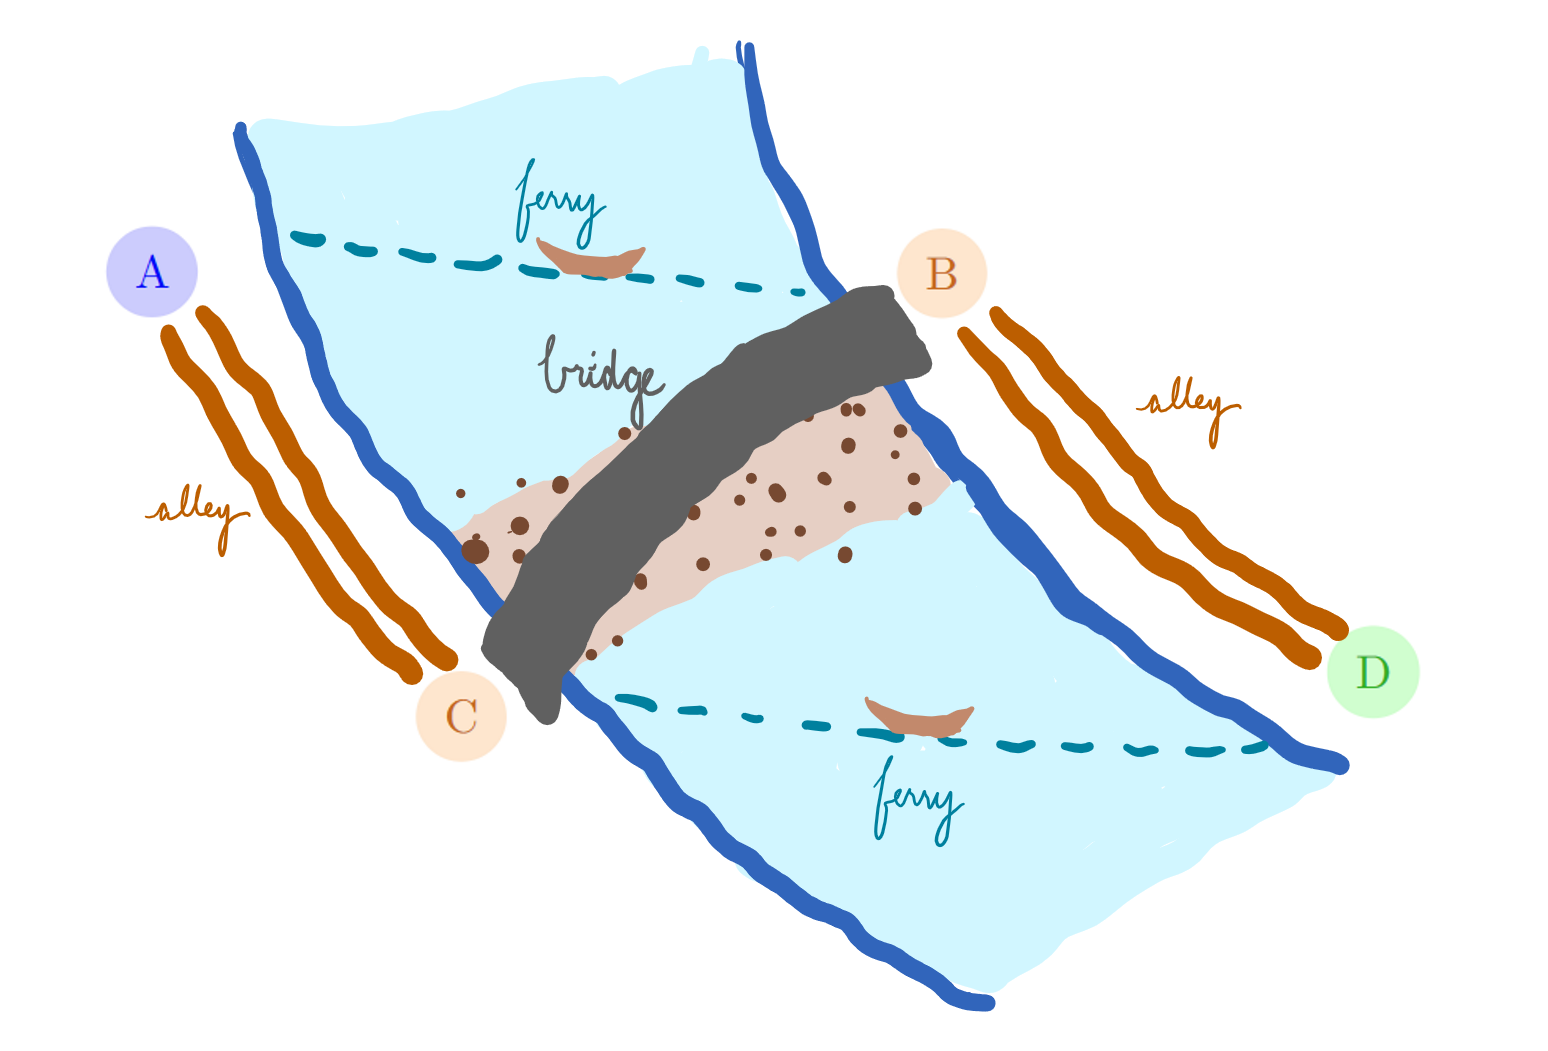
\includegraphics[width=0.6\linewidth]{images/Venice_bridge_crossing_illustration.png}
    \caption{Illustration of paths available to cross the Grand Canal}
    \label{fig:veniceill}
\end{figure}

A diagram for the paths available is shown in Figure~\ref{fig:bp_frame}. \nodeA~is the start node and \nodeD~is the end node. The nodes in between are \nodeB~and \nodeC. We have named the paths too, for convenience: \nodeA\nodeB~and \nodeC\nodeD~are \pathferry~paths, and \nodeB\nodeD~and \nodeA\nodeC~are \pathalley~paths. \nodeB\nodeC~is the \pathbridge~path which is connected later and causes an increase in time taken for the \NE.

\begin{figure}[htbp]
    \centering
    \bpdiag{\alpha}{\beta}{\delta}
    \caption{Basic framework for illustrating \bp}
    \label{fig:bp_frame}
\end{figure}

\subsection{Setting up the game}

\begin{table}[htbp]
    \centering
    \begin{tabular}{|c|c|}
    \hline
       $\alpha$  & Time taken on the \pathferry \\ \hline
       $\beta$  & Time taken on the \pathalley \\ \hline
       $\delta$  & Extra time taken on the \pathalley~for every person on the \pathalley\\ \hline
       $n$  & Number of agents in the game \\ \hline
    \end{tabular}
    \caption{Parameters of the \bp~game}
    \label{tab:bpParams}
\end{table}

We need to choose the parameters in Table \ref{tab:bpParams} such that the all the agents take the alley-bridge-alley path at the \NE, and this is higher than the \NE~cost for the case without the bridge. Therefore, the following costs need to be in descending order:

\begin{enumerate}
    \item Time taken on the \pathferry-\pathbridge-\pathferry~route ($2\alpha$)
    \item Time taken on the \pathferry-\pathbridge-\pathalley~route ($\alpha+\beta+\delta n_{\text{\nodeB\nodeD}}$, $\alpha+\beta+\delta n_{\text{\nodeA\nodeC}}$)
    \item Time taken on the \pathalley-\pathbridge-\pathalley~route ($2\beta+\delta(n_{\text{\nodeB\nodeD}}+n_{\text{\nodeA\nodeC}})$)
    \item Time taken on the \pathalley-\pathferry~route in the case without the \pathbridge~connected 
\end{enumerate}

In the case without the bridge connected, let us consider unequal numbers of agents taking either of the routes \nodeA\nodeB\nodeD~or \nodeA\nodeC\nodeD. Then the number of people on a particular route will be higher, increasing the time taken on that route. None of the agents would want to change routes when the cost on either route is equal, that is, the number taking either route is the same $=n/2$.

Furthermore, from the symmetry of the game, let us assume that the number of people taking \pathferry-\pathbridge-\pathalley~and \pathalley-\pathbridge-\pathferry~are the same, and therefore, $$n_{\text{\nodeA\nodeB\nodeD}}=n_{\text{\nodeA\nodeC\nodeD}} \implies n_{\text{\nodeA\nodeB\nodeD}} + n_{\text{\nodeA\nodeC\nodeB\nodeD}}=n_{\text{\nodeA\nodeC\nodeD}}+ n_{\text{\nodeA\nodeC\nodeB\nodeD}} \implies n_{\text{\nodeB\nodeD}} = n_{\text{\nodeA\nodeC}} =n'$$

Therefore we need the following inequality to be satisfied:
$$ 2\alpha> \alpha+\beta+\delta n'> 2\beta+2\delta n'>\alpha+\beta+\delta \frac{n}{2}$$
which simplifies to $$n'>\frac{n}{2} \And \alpha>\beta+\delta n' \And 2n'-\frac{n}{2}>\frac{\alpha-\beta}{\delta}$$
now allowing all the agents to take the \pathalley~routes (setting $n'=n$) we have $$n<\frac{\alpha-\beta}{\delta}<\frac{3}{2}n$$

A set of parameters that obeys this rule is $(\alpha=15, \beta=2, \delta=0.2, n=60)$. These parameters make sense in our setting of the Grand Canal crossing in Venice. We have also considered the parameter set $(\alpha=40, \beta=15, \delta=0.1, n=200)$. The costs and price of anarchy due to this setup is shown in Table~\ref{tab:bpCostspoa}.

\begin{table}[htbp]
    \centering \small
    \begin{tabular}{|c|c|c|} \hline
         & $(\alpha=15, \beta=2, \delta=0.2, n=60)$ & $(\alpha=40, \beta=15, \delta=0.1, n=200)$ \\ \hline
        Cost at NE without \pathbridge~(\nodeA\nodeB\nodeD, \nodeA\nodeC\nodeD) & (23, 23) & (65, 65)\\
        Cost at NE (\nodeA\nodeB\nodeD, \nodeA\nodeC\nodeD, \nodeA\nodeB\nodeC\nodeD, \nodeA\nodeC\nodeB\nodeD) & (29, 29, 30, 28) & (75, 75, 80, 70) \\
        Price of Anarchy & $\frac{28}{22.96}=121.95\%$ & $\frac{70}{64.375}=108.74\%$ \\ \hline        
    \end{tabular}
    \caption{Costs and Price of Anarchy with different parameter choices}
    \label{tab:bpCostspoa}
\end{table}

We consider the infinite repetition of the above described game in which the route selection is posed infinitely over multiple stages. For simulation purposes and developing the algorithm, we consider a high number $K$ that represents a finitely large number of stages. 

\subsection{Preliminary Agent Model}\label{sub:PAM}
Initially we model all the agents to be identical and possess two different parameters namely,
\begin{itemize}
    \item \textbf{Selfishness $\gamma$}: $\gamma \in [0,1]$ defines how selfish an agent is. $\gamma = 0$ indicates that the agent is completely selfish while $\gamma = 1$ indicates that the agent is completely benevolent. 
    \item \textbf{Connectivity $|\mathcal{N}|$}: Connectivity defines how well-connected an agent is. $\mathcal{N}$ is a set that comprises of all the the ``neighbours" of the agent. The higher the number of neighbours, the more well-connected the agent is considered to be.
\end{itemize}

We can model the cost that each agent is trying to minimize at stage $s$ of the game to be,
\begin{align}
    J_i(s,a_1, \cdots a_n) =(1-\gamma) C_i(s,a_1, \cdots a_n) +  \gamma\sum\limits_{l \in \mathcal{N}}C_l(s,a_1, \cdots a_n)
\end{align}

where $C_i(s,a_1, \cdots a_n)$ represents the time taken by an agent to reach the destination from the source, given the actions of all the agents $a_1, \cdots a_n$.

\subsection{Centralized Scheduler}
The Centralized Scheduler (CS) has been modelled as an entity, different from the agents that play the game, to regulate the state of affairs. The two major responsibilities of the Centralized Scheduler are
\begin{itemize}
    \item to decide the $\gamma$ and $|\mathcal{N}|$ values for the agents
    \item to schedule/prioritize the agents based on the cost they incur at every stage of the game
\end{itemize}

Figure \ref{fig:CS_Arch} represents how the communication would happen in the presence of a Centralized Scheduler. The agents would all communicate with the CS and there would be no inter-agent communication. Figure \ref{fig:IE} on the other had represents the information that is actually exchanged between the agent and the CS. While the CS transmits the selfishness, connectivity and the time that all the neighbours of an agent would collectively take in order to reach the destination to the agents, each agent would in turn transmit the cost it incurs to the CS. 

\begin{figure}[htbp]
    \centering
    \begin{subfigure}[c]{0.45\linewidth}
        \centering
        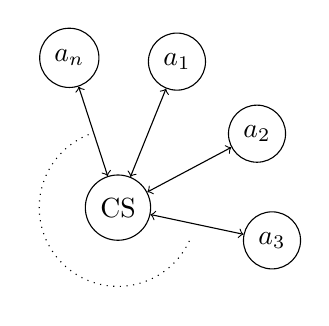
\begin{tikzpicture}
        \label{star_poa}
        \def \n {20}
        \def \N {8}
        \def \radius {2cm}
        \def \rd {1mm}
        \def \rer {4mm}
        
        \def \margin {8} % margin in angles, depends on the radius
        
        \node[draw, circle] at (360:0mm) (ustar) {CS};
        \foreach \i [count=\ni from 0] in {n,1,2,3}{
          \node[draw, circle] at ({108-\ni*40}:\radius) (u\ni) {$a_{\i}$};
          \node at ({115-\ni*40}:\radius/2) {};
          \draw[<->] (ustar)--(u\ni);
        }
        
        \draw[dotted,black] (-25:\radius/2) arc[start angle=-25, end angle=-250, radius=\radius/2];
        \end{tikzpicture}
        \caption{Centralized Scheduler Architecture}
        \label{fig:CS_Arch}
    \end{subfigure}
    \hfill
    \begin{subfigure}[c]{0.45\linewidth}
        \centering
        \scalebox{0.8}{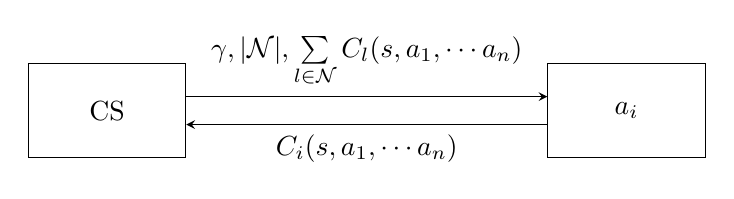
\begin{tikzpicture}
        % CS
        \node [draw,
            minimum width=2cm,
            minimum height=1.2cm,
        ]  (centralscheduler) at (0,0){CS};
         
        % Agent
        \node [draw, 
            minimum width=2cm, 
            minimum height=1.2cm,
        ] (agent) at (6.6,0){$a_i$};

        \draw[-stealth] (centralscheduler.10)--(centralscheduler.10-|agent.west) 
        node[midway,above]{$\gamma,|\mathcal{N}|,     \sum\limits_{l \in \mathcal{N}}C_l(s,a_1, \cdots a_n)$};
        \draw[-stealth] (agent.-170)--(agent.-170-|centralscheduler.east) 
        node[midway,below]{$C_i(s,a_1, \cdots a_n)$};
        \end{tikzpicture}}
        \caption{Information Exchange}
        \label{fig:IE}
    \end{subfigure}
    \caption{Architecture and information exchange for the Centralized Scheduler}
    \label{fig:CSArchandIE}
\end{figure}



\begin{algorithm}[H]
\caption{$C(a_1, \cdots a_n) = \text{CentralizedSchedulerArchitecture}(\gamma,|\mathcal{N}|,     \sum\limits_{l \in \mathcal{N}}C_l(a_1, \cdots a_n))$}\label{alg:nealg}
\begin{algorithmic}[1]
\State Receive $\gamma$ and $\mathcal{N}$ from CS
\For{$s = 1 \cdots K$}
    \State $prev_{a_i} \gets None, \forall i \in [n]$
    \State $a_i \gets \nodeA\nodeB\nodeD, \forall i \in [n]$
    \While{$prev_{a_i} \neq a_i$}
        \For{$i= 1 \cdots n$}
        \State $prev_{a_i} \gets a_i$
        \State $a_i = \argmin\limits_{a_i} (1-\gamma) C_i(s,a_1, \cdots a_n) +  \gamma\sum\limits_{l \in \mathcal{N}}C_l(s,a_1, \cdots a_n)$
        \EndFor
    \EndWhile
    \State $C(a_1, \cdots a_n)[s][i] \gets C_i(s,a_1, \cdots a_n)$
    \State CS sorts $C_i(s,a_1, \cdots a_n)$ values in descending order
    \State CS assigns $i$ based on the sorted order
\EndFor
\end{algorithmic}
\end{algorithm}

The above Algorithm \ref{alg:nealg} illustrates the working of the CS based setup. Initially, the CS decides the parameters for the agents that are fixed for all stages of the game. Then, at each stage of the game, the agents initialize to random actions and try to choose the action that minimizes their costs while constantly exchanging information with the CS. Once all the agents iterate and finalize their actions, they incur a cost which they communicate to the CS. The CS then orders the agents such that at the next stage of the game $s+1$, the agents with a high cost at the current stage $s$ get the opportunity to decide their action first. 

\subsection{Dynamic Agent Model}\label{sub:DAM}
Although the Centralized Scheduler and the Preliminary Agent Model work in overcoming the paradox on average as we would see in Section \ref{sec:results}, certain characterstics of this model make it undesirable. For instance, all the decisions are controlled by one entity, which is the CS in the previous model. Moreover, the agents are not allowed to act independently and choose their own actions. Finally, the agents may simply not follow the directions obtained from the CS and thus the model might not work practically. For this reason, we desire a distributed model that overcomes all the said shortcomings, while still trying to overcome the paradox which is our primary goal. 

We propose the Dynamic Agent Model in which the agents have full control over the parameters introduced in Section \ref{sub:PAM}. In the absence of the Centralized Scheduler, the aim of this model is for the agents to update their selfishness $\gamma_i(t)$ and connectivity parameters  $\mathcal{N}_i(t)$ over the stages of the game in a meaningful way, while also making sure that all the agents get a fair chance to overcome the paradoxical situation. 

Intuitively, it is easy to see that if an agent $i$ experiences a ``high" cost at stage $s-1$, then it indicates that the agent has not been ``selfish" enough in $s-1$. Thus, for the agent to be benefited at stage $s$, it needs to reduce its selfishness and connectivity parameters. While on the other hand if the agent incurs only a ``low" cost at stage $s-1$, then the agent has been more selfish in that stage and in order to give a fair chance to all the other agents, the agent should decide to be more benevolent and more connected to its neighbours in the upcoming stage than the current stage. 

A working heuristic for the dynamics of the parameters is 
\begin{align}\label{eqn:dynamicsheuristic}
     \text{If} \quad &J_i(t-1) > \tau\nonumber\\
        \quad&\gamma_i(t) = \max(0,\gamma_i(t-1)/4)\nonumber\\
        \quad&|\mathcal{N}_i(t)| = \max(0,|\mathcal{N}_i(t-1)|/4)\nonumber\\
      \text{Else}&\nonumber\\
        \quad&\gamma_i(t) = \min(1,2\gamma_i(t-1))\nonumber\\
        \quad&|\mathcal{N}_i(t)| = \min(n,2|\mathcal{N}_i(t-1)|)        
\end{align}

where $\tau$ is the cost threshold that indicates if a cost incurred is high or low. An ``informed" decision of $\tau$ can be made by the agents based on the NE cost they used to incur prior to the construction of the bridge.

\subsection{Distributed Architecture}
As remarked in Section \ref{sub:DAM}, the centralized scheduler and approach have some limitations to be addressed, leading to a distributed approach. As illustrated in Figure~\ref{fig:DAdetails} in this architecture, the an agent $i$ receives information from its neighbours in $\mathcal{N}_i$ directly, while transmitting the time they would take to reach the destination to all the agents that consider agent $i$ to be their neighbour. It is to be noted that an agent $i$ need not necessarily consider another agent $j$ to be its neighbour, just because agent $j$ considers agent $i$ to be its neighbour.

\begin{figure}[htbp]
    \centering
    
\begin{subfigure}{\linewidth}
    \centering
    \DAarch{0}{1}{2}{3}
    \DAarch{1}{2}{5}{7}
    \DAarch{n}{0}{3}{n-1}    
    \caption{Distributed Architecture}
    \label{fig:DAarchitecture}
\end{subfigure}

\begin{subfigure}{0.6\linewidth}
    \centering
    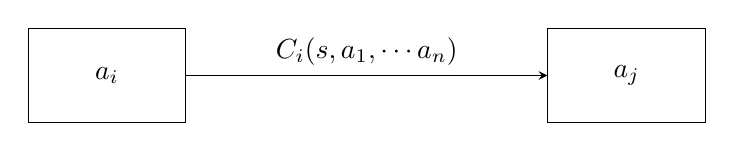
\begin{tikzpicture}
    % a1
    \node [draw,
        minimum width=2cm,
        minimum height=1.2cm,
    ]  (ai) at (0,0){$a_i$};
     
    % a2
    \node [draw, 
        minimum width=2cm, 
        minimum height=1.2cm,
    ] (aj) at (6.6,0){$a_j$};

    \draw[-stealth] (ai.east)--(aj.west) 
    node[midway,above]{$C_i(s,a_1, \cdots a_n)$};
    \end{tikzpicture}
    \caption{Information Exchange in Distributed Architecture}
    \label{fig:DAie}
\end{subfigure}

    \caption{Details of the Distributed Architecture}
    \label{fig:DAdetails}
\end{figure}

        
\begin{algorithm}[H]
\caption{$C(a_1, \cdots a_n) = \text{DistributedArchitecture}(\tau)$}\label{alg:nealgdistr}
\begin{algorithmic}[1]
\State Initialize $\gamma_i(1) \sim \mathcal{U}(0,1), \forall i \in [n]$
\State Initialize $|\mathcal{N}_i(1)| \sim \mathcal{U}(0,n), \forall i \in [n]$
\For{$s = 1 \cdots K$}
    \State $prev_{a_i} \gets \text{None}, \forall i \in [n]$
    \State $a_i \gets \nodeA\nodeB\nodeD, \forall i \in [n]$
    \If{$s > 1$}
        \If{$J_i(s-1,a_1,\cdots,a_n) > \tau$}
            \State $\gamma_i(t) = \max(0,\gamma_i(t-1)/4)$
            \State $|\mathcal{N}_i(t)| = \max(0,|\mathcal{N}_i(t-1)|/4)$
        \Else
            \State $\gamma_i(t) = \min(1,2\gamma_i(t-1))$
            \State $|\mathcal{N}_i(t)| = \min(n,2|\mathcal{N}_i(t-1)|$
        \EndIf
    \EndIf
    \While{$prev_{a_i} \neq a_i$}
        \For{$i= 1 \cdots n$}
        \State $prev_{a_i} \gets a_i$
        \State $a_i = \argmin\limits_{a_i} (1-\gamma) C_i(s,a_1, \cdots a_n) +  \gamma\sum\limits_{l \in \mathcal{N}}C_l(s,a_1, \cdots a_n)$
        \EndFor
    \EndWhile
    \State $C(a_1, \cdots a_n)[s][i] \gets C_i(s,a_1, \cdots a_n)$
\EndFor
\end{algorithmic}
\end{algorithm}

The above Algorithm \ref{alg:nealgdistr} depicts the simulation of the system based on the dynamic agent model and the distributed architecture. We initialize the selfishness and connectivity parameters to a random value sampled from a uniform distribution. Then at each stage of the game, the agents update their parameters based on the dynamics described in equation \ref{eqn:dynamicsheuristic}; followed by which the agents iterate over their best responses until they converge to an action.  

\section{Simulation Results and Discussion}\label{sec:results}
In this section we look at and compare the results obtained from the Centralized Scheduler and the Distributed Architecture. The parameters that we have used for the simulation are $(\alpha=40, \beta=15, \delta=0.1, n=200)$ with an NE cost of 65 without the bridge and 70 with the bridge, amounting to a Price of Anarchy of 108.74\% as stated in Table \ref{tab:bpCostspoa}. We simulate the multistage game for $K=1000$ stages. 

The two major values that we consider in our results are $J_{avg}$ and $J_{i, \text{avg}}$. $J_{avg}$ is the average cost incurred per agent per stage of the game. $J_{i, \text{avg}}$ is the average cost incurred by an agent $i$ over the stages of the game. $J_{avg}$ indicates the overall welfare of all the agents, whereas $J_{i, \text{avg}}$ indicates the welfare of each agent over the stages of the game. We would need the agents to have similar welfare and not favour any particular group of agents.
\subsection{Centralized Scheduler}
We study the results of the CS Architecture Algorithm depicted in Algorithm \ref{alg:nealg}. Figure \ref{fig:results_central_scheduler_plot} shows the variation of $J_{avg}$ with respect to $\gamma$ and $|\mathcal{N}|$ values selected by the CS. It is clear that for low values of $\gamma$ and $|\mathcal{N}|$, the average cost per agent per stage $J_{avg}$ remains high at 70, which is the NE cost value. However the lowest value obtained is 64.375  for $\gamma =1$ and $|\mathcal{N}|=200$. This is lower than the value of 65 which is the NE value prior to the construction of the bridge. This result reaffirms the fact that if agents do not play selfishly, but rather coordinate with other agents they can overcome the paradox.
\begin{figure}[htbp]
    \centering
    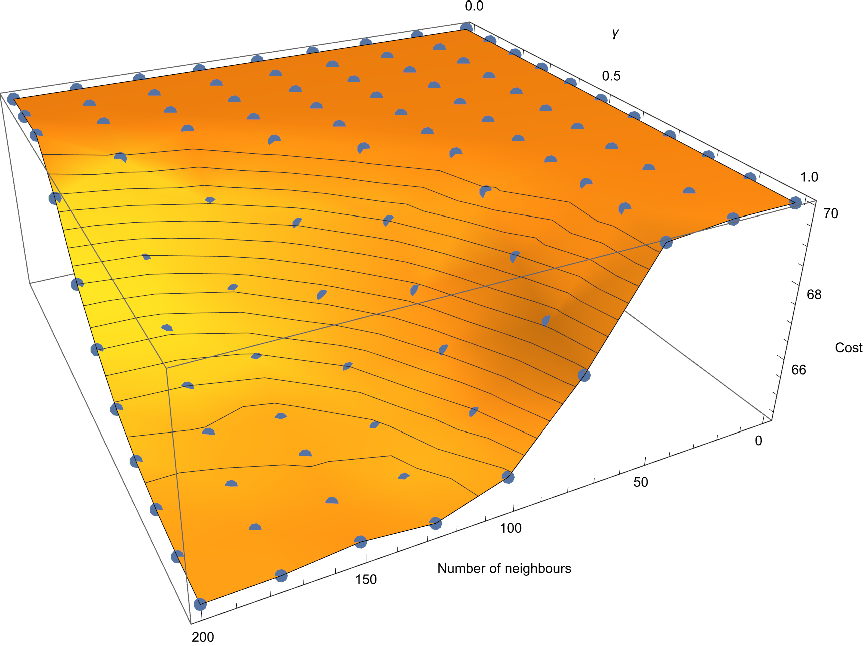
\includegraphics[width=0.7\linewidth]{images/CS_costs.pdf}
    \caption{Variation of $J_{avg}$}
    \label{fig:results_central_scheduler_plot}
\end{figure}

We then plot the average costs incurred by the agents over the stages of the game. Figure \ref{fig:results_central_scheduler_avg_player_no_random} shows the case when the CS inadvertently favours a group of agents while assigning the priority values when the agents incur the same cost. This effect can be mitigated by introducing a randomization when the CS assigns priority to agents that incur the same cost in the current stage of the game. Figure \ref{fig:results_central_scheduler_avg_player_random} shows that the agents incur similar average costs over the stages and as $K$ increases, the difference in costs between the agents would reduce. 

\begin{figure}[htbp]
\centering
\begin{subfigure}[c]{0.49\linewidth}
    \centering
    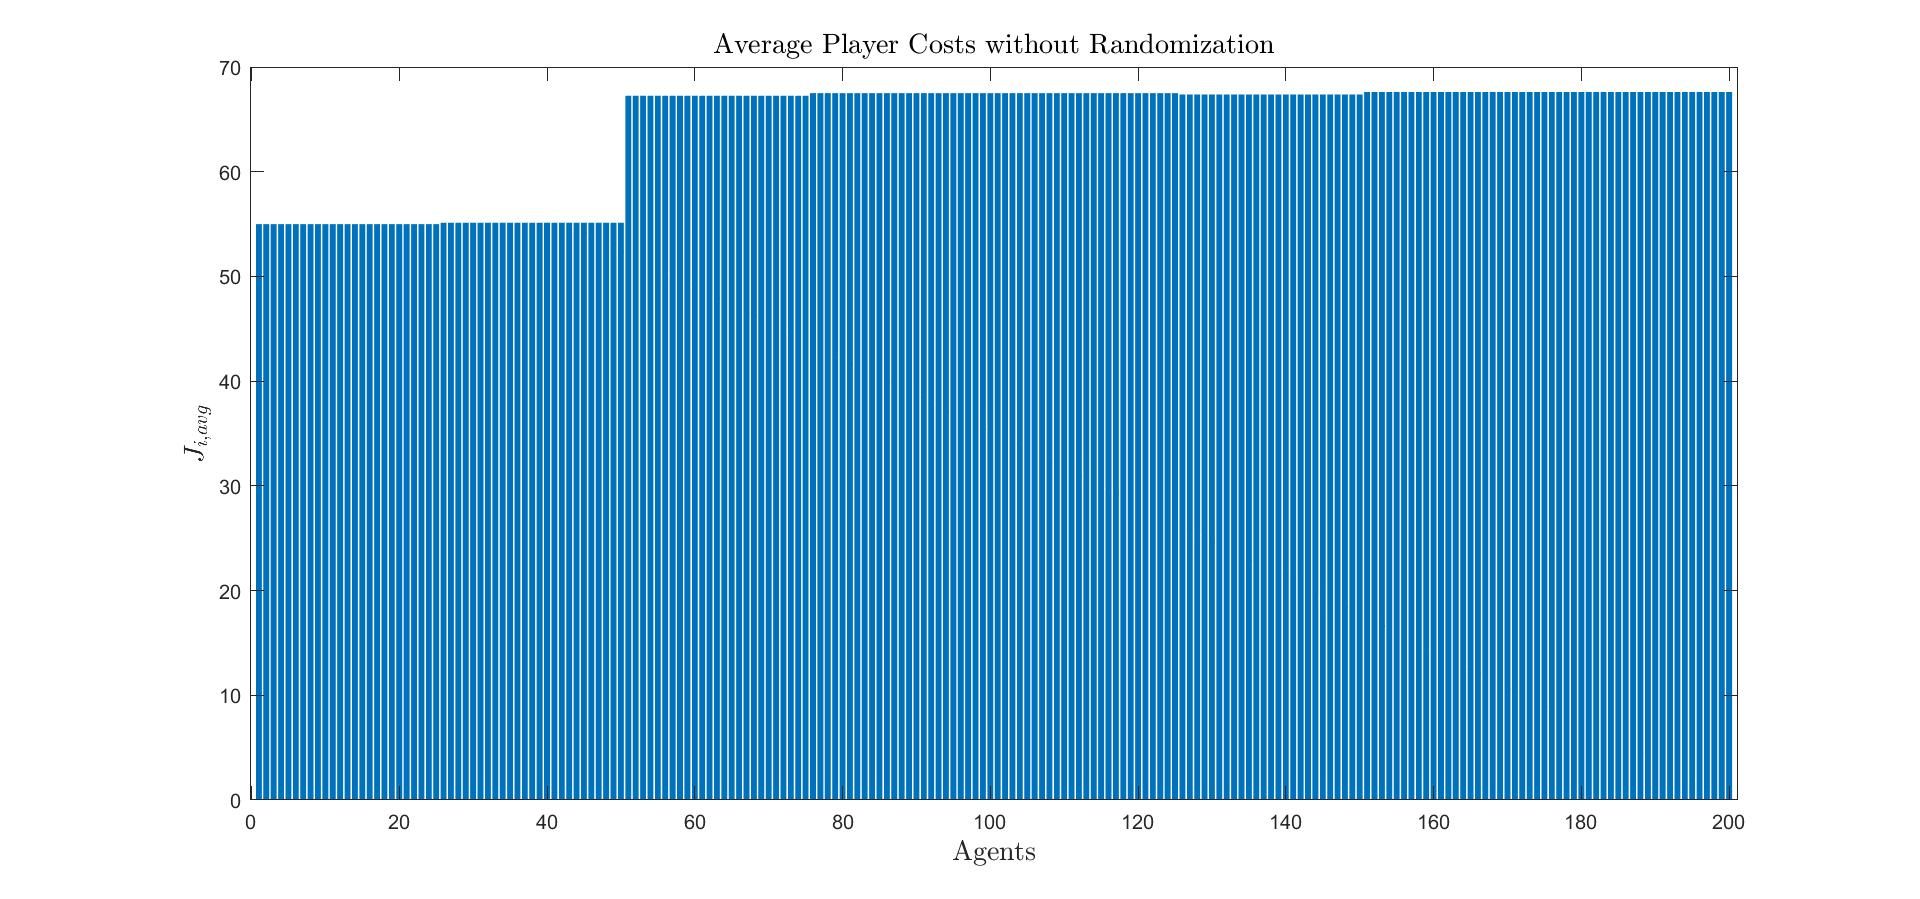
\includegraphics[width=\linewidth, trim=150 0 150 0, clip]{images/results_central_scheduler_avg_player_no_random.jpg}
    \caption{Without randomized priority in scheduling}
    \label{fig:results_central_scheduler_avg_player_no_random}
\end{subfigure}
\hfill
\begin{subfigure}[c]{0.49\linewidth}
    \centering
    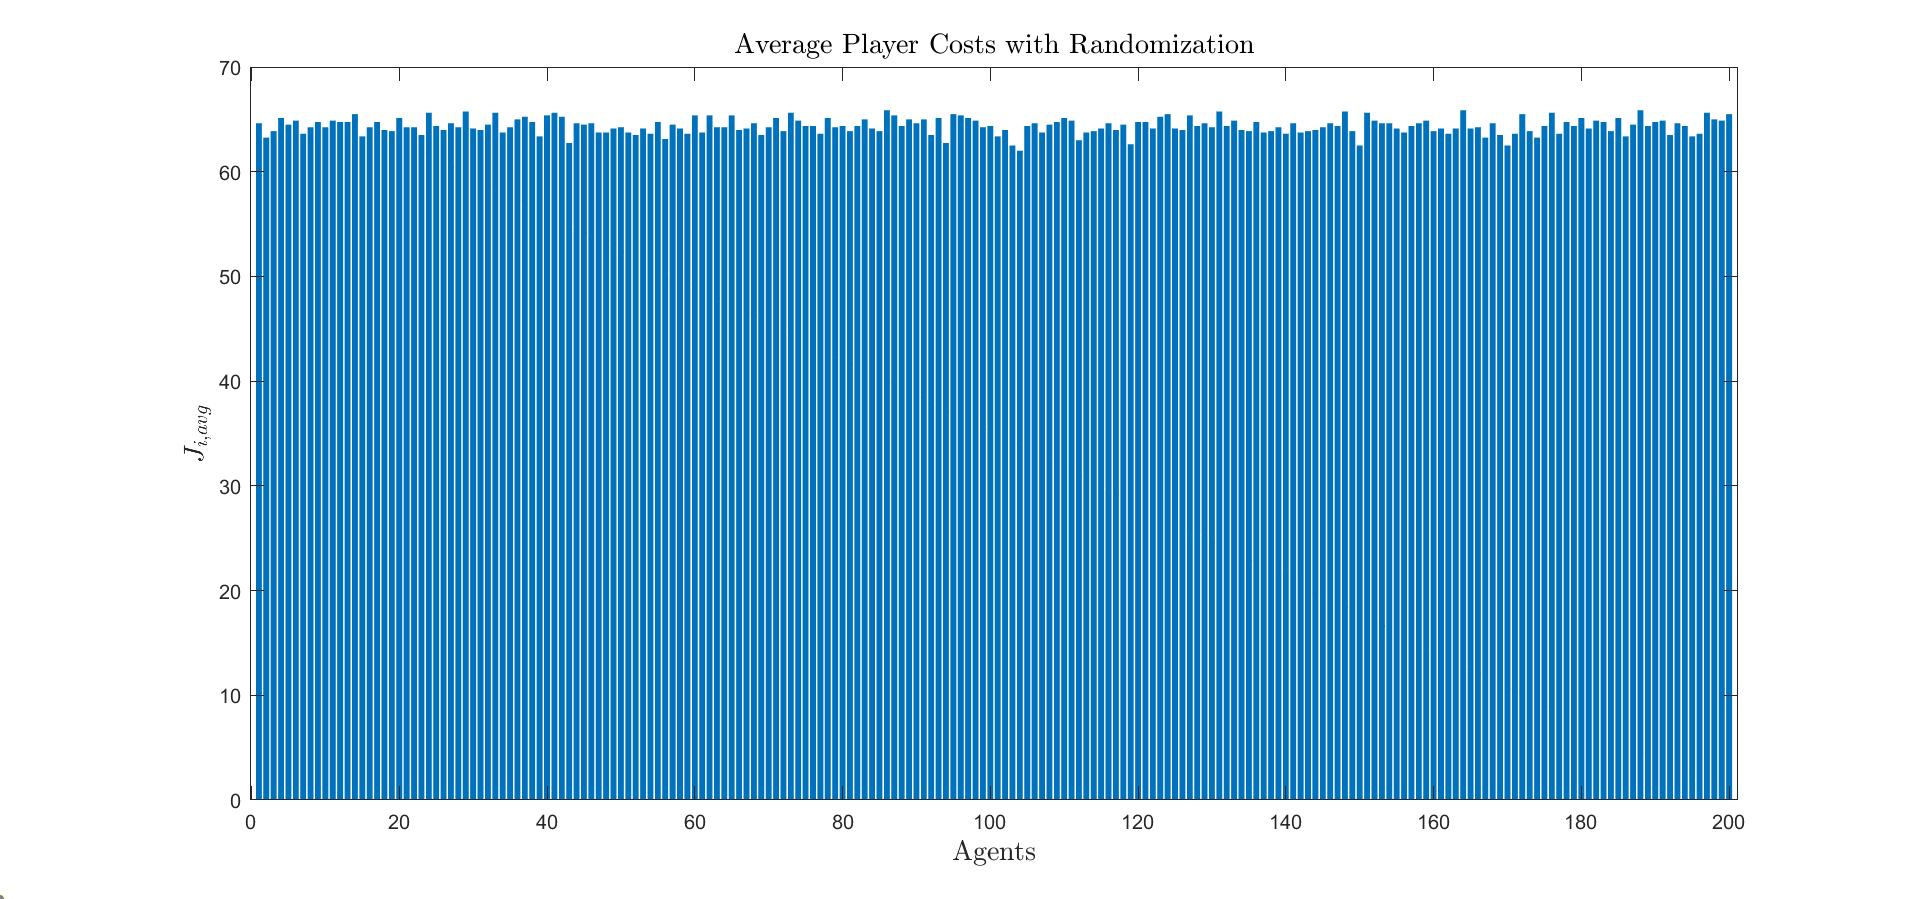
\includegraphics[width=\linewidth, trim=150 0 150 0, clip]{images/results_central_scheduler_avg_player_random.jpg}
    \caption{With randomized priority in scheduling}
    \label{fig:results_central_scheduler_avg_player_random}
\end{subfigure}
\caption{Variation in $J_{i, \text{avg}}$ based on scheduling priority}
\label{fig:results_central_scheduler_avg_player}
\end{figure}

\subsection{Distributed Architecture}
In this subsection we study the results of the Distributed Architecture based algorithm that is outlined in Algorithm \ref{alg:nealgdistr}. After conducting Monte Carlo Study with 200 trials, Figure~\ref{fig:results_distributed_avg_cost} shows the value of $J_{avg}$ over the trials. It can be observed that $J_{avg} \sim \mathcal{N}(64.515, 0.016)$. The mean over the trials is 64.515 is lower than 65 which is the NE value prior to the construction of the bridge. This indicates that the paradoxical situation can be avoided with the proposed dynamic agent model on average over different stages of the game. 
\begin{figure}[htbp]
    \centering
    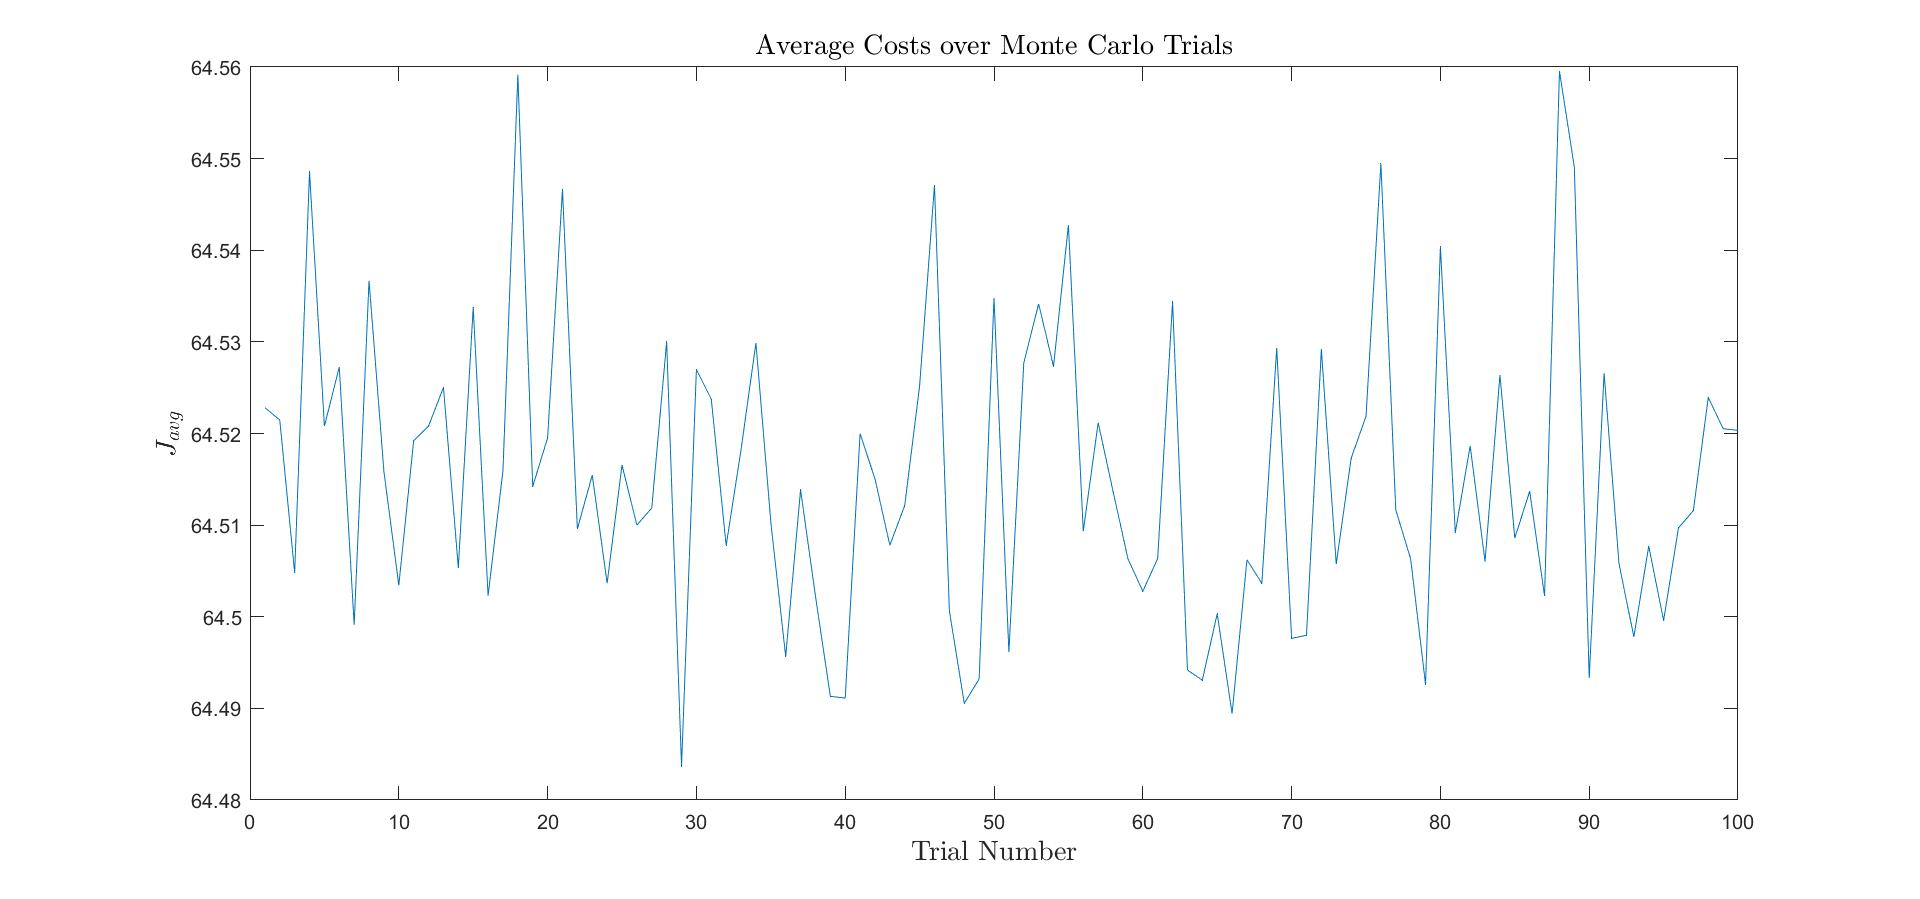
\includegraphics[width=\linewidth]{images/results_distributed_avg_cost.jpg}
    \caption{Average Costs - Results of Monte Carlo Trials with $\gamma_i(0) \sim \mathcal{U}(0,1)$ and $|\mathcal{N}_i(0)| \sim \mathcal{U}(0,200)$}
    \label{fig:results_distributed_avg_cost}
\end{figure}
We would also like to look at how the average agent costs is distributed over the trials. Clearly, from Figure \ref{fig:results_distributed_avg_player_cost}, it can be inferred that the costs of agents are distributed more or less uniformly except for some anomalies that arise due to the approximation to a finite number of stages.
\begin{figure}[htbp]
    \centering
    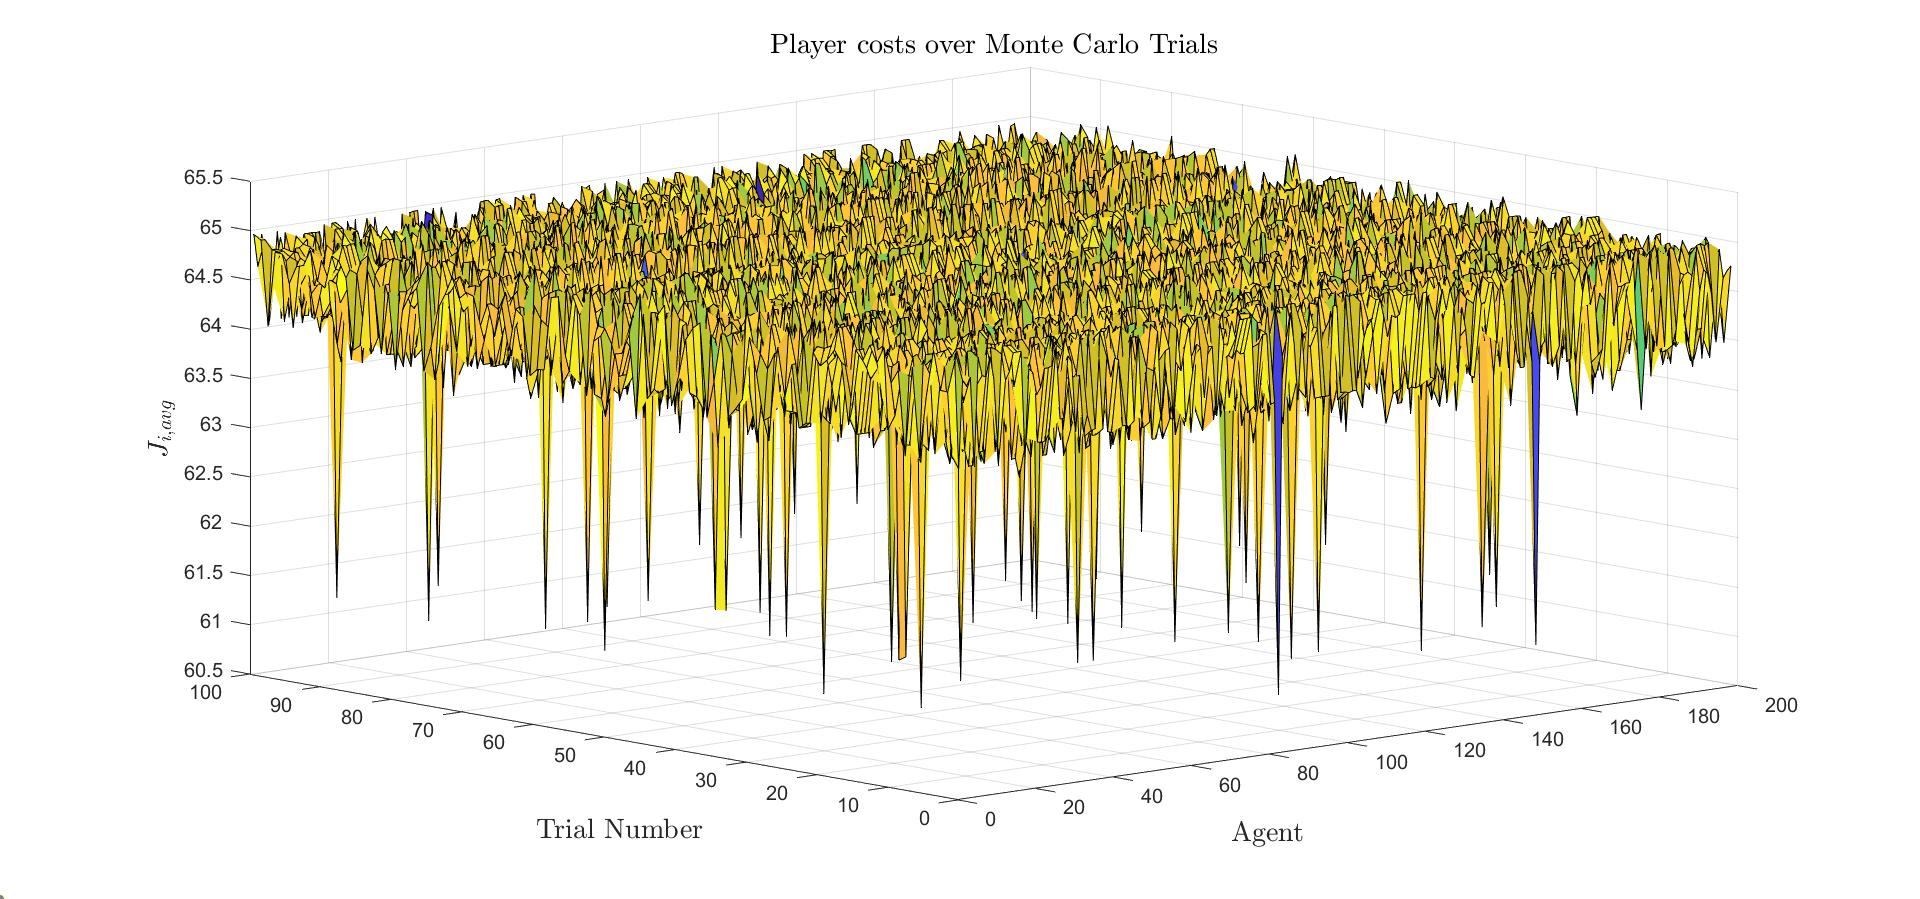
\includegraphics[width=\linewidth]{images/results_distributed_avg_player_cost.jpg}
    \caption{Average agent Costs - Results of Monte Carlo Trials with $\gamma_i(0) \sim \mathcal{U}(0,1)$ and $|\mathcal{N}_i(0)| \sim \mathcal{U}(0,200)$}
    \label{fig:results_distributed_avg_player_cost}
\end{figure}
It would also be important to look into the dynamics of the agent parameters $\gamma_i(s)$ and $|\mathcal{N}_i(s)|$ and how it evolves over stages since they are specific to each agent. It is inferred from the observations that after a number of stages of the game has passed, most of the agents can be grouped together based on their parameter dynamics. Figure \ref{fig:results_distributed_player_gamma} shows the evolution of $\gamma_i(t)$ for three such groups. It can be seen that the values oscillate between 0.25, 0.5 and 1 and it converges to a ``limit cycle" like behaviour. Similar is the case with the dynamics of $|\mathcal{N}_i(s)|$  depicted in Figure \ref{fig:results_distributed_player_neighbours}. The final 11 stages are depicted in the figures for clarity.

\begin{figure}[htbp]
    \centering
    \begin{subfigure}[c]{0.49\linewidth}
    \centering
    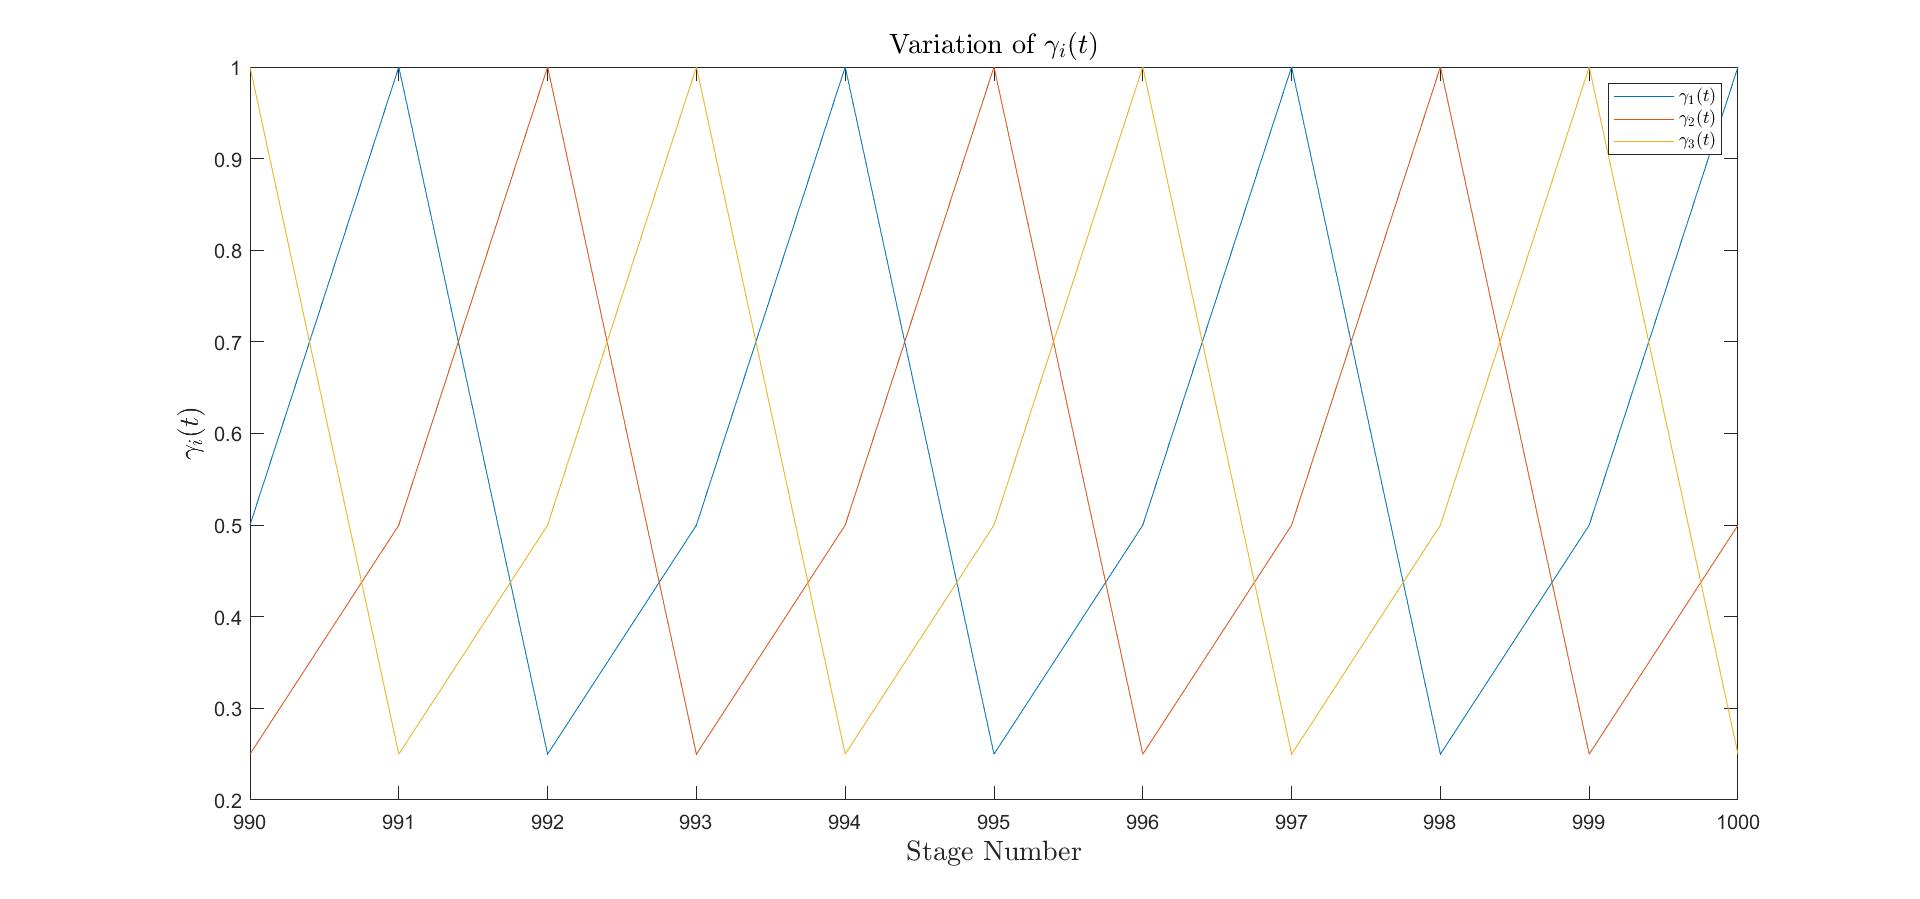
\includegraphics[width=\linewidth, trim=150 0 150 0, clip]{images/results_distributed_player_gamma.jpg}
    \caption{Variation of $\gamma$ with stage}
    \label{fig:results_distributed_player_gamma}
\end{subfigure}
\hfill
\begin{subfigure}[c]{0.49\linewidth}
    \centering
    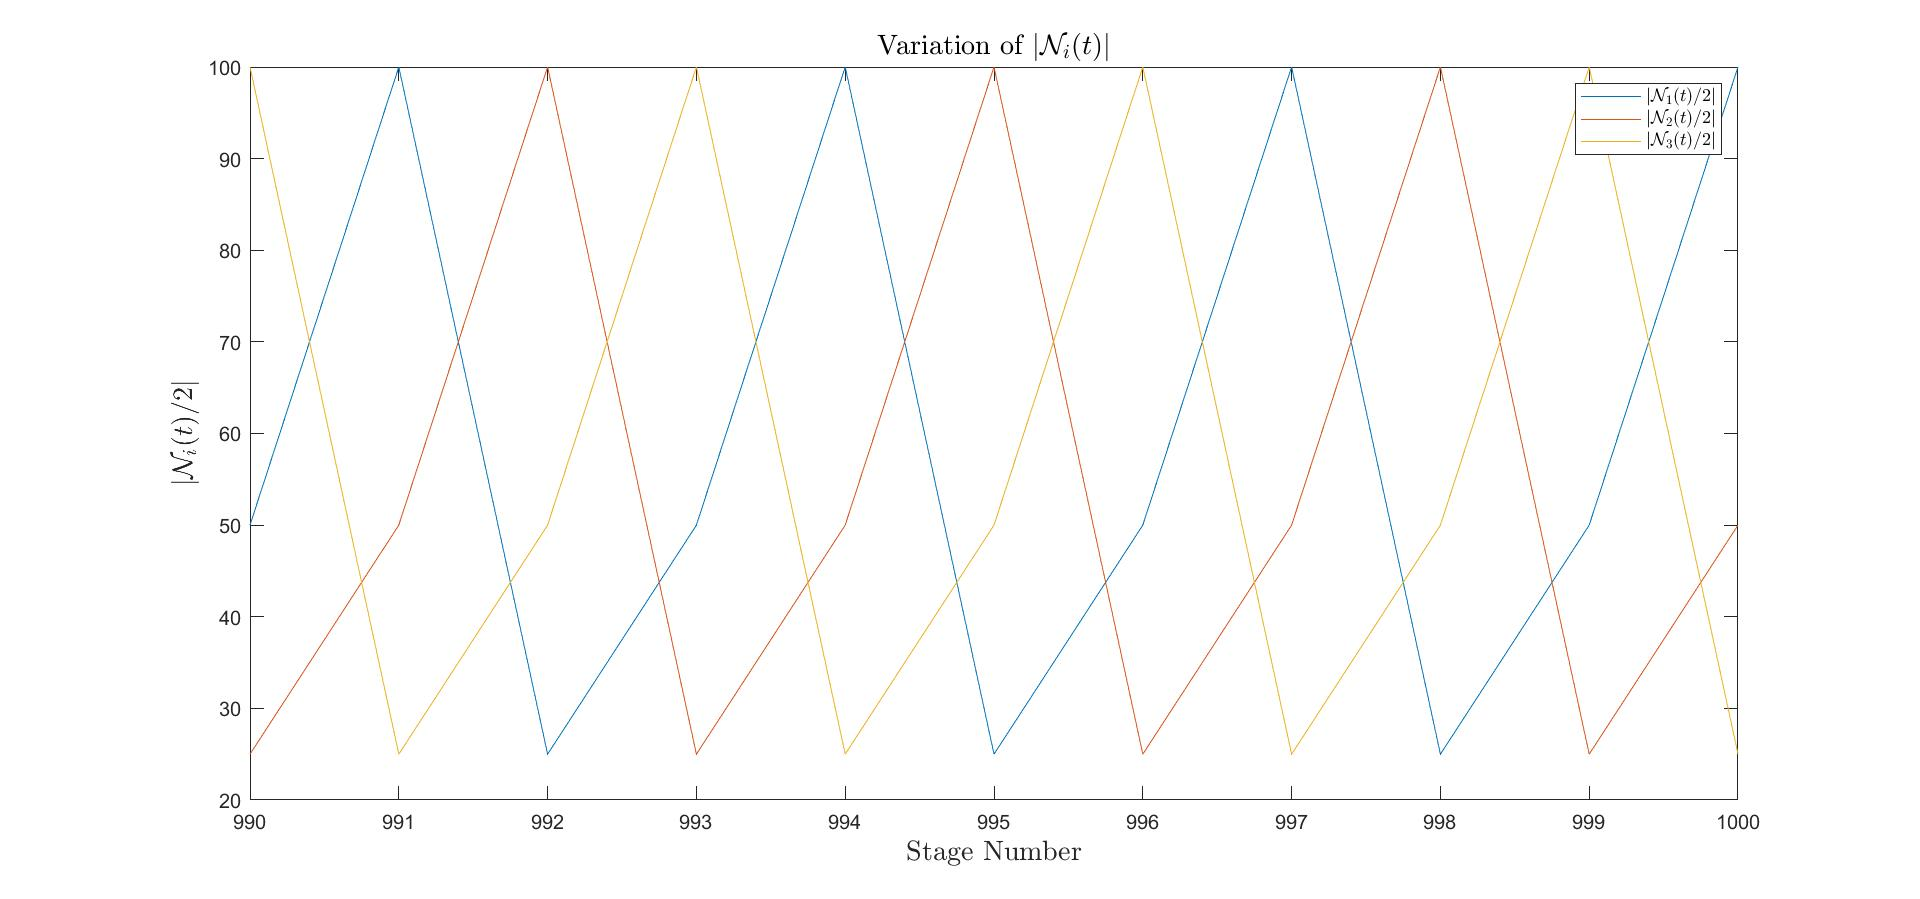
\includegraphics[width=\linewidth, trim=150 0 150 0, clip]{images/results_distributed_player_neighbours.jpg}
    \caption{Variation of $|\mathcal{N}|$ with stage}
    \label{fig:results_distributed_player_neighbours}
\end{subfigure}
    \caption{Variation of agent parameters with stage}
    \label{fig:results_distributed_player}
\end{figure}

\begin{figure}[htbp]
    \centering
    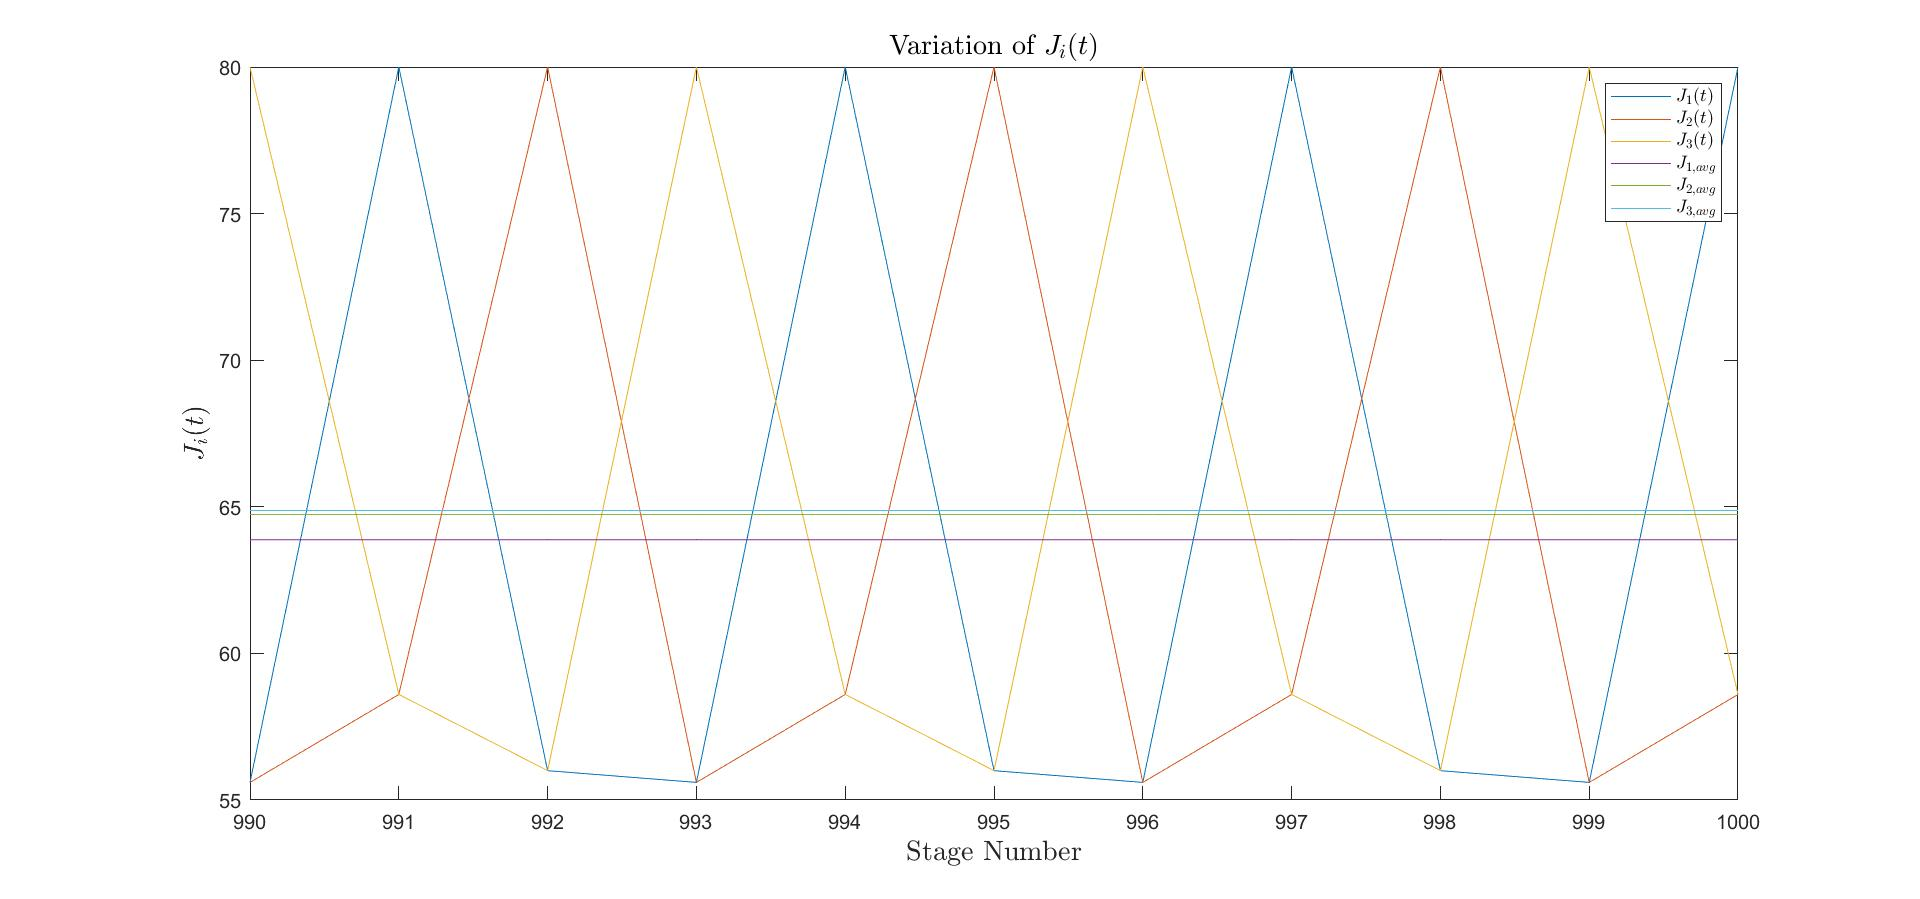
\includegraphics[width=\linewidth]{images/results_distributed_player_cost.jpg}
    \caption{Individual agent Cost Behaviour with $\gamma_i(0) \sim \mathcal{U}(0,1)$ and $|\mathcal{N}_i(0)| \sim \mathcal{U}(0,200)$}
    \label{fig:results_distributed_player_cost}
\end{figure}

Finally, we look at costs incurred by the three largest groups and we can see that they incur pretty low costs (lesser than 65) for two stages and one high cost (80) due to the agents being modelled to be reasonable. Clearly, we can see that the average costs are lower than 65 on average, thus reducing the time taken on average to get to the destination from the source after the construction of the bridge. 

\section{Conclusion and Outlook}
It is a known fact that selecting a route selfishly might not always lead to the minimum possible cost that can be achieved and from our simulations we are clearly able to reiterate the fact. A Centralized Scheduler based Architecture might be able to mitigate the effect and overcome the paradox under the assumption that the Scheduler always acts in a fair manner and all the agents abide by the rules set by the Centralized Scheduler. The shortcomings however with this method outweigh the advantages which makes us investigate as to how the agents can themselves take rational decisions independently to overcome the paradox. The proposed Dynamic Agent Model along with the heuristics for the dynamics of the agent parameters achieves this as outlined in the results. Thus, modelling the agents reasonably, \textbf{helps overcome Braess's Paradox on average in an infinitely repeated game}.

Further directions of investigations would be to take practical considerations into account. Human beings might not be able to fit into the proposed Dynamic Agent Model; however smartphone apps that perform the route selection on behalf of the human beings could be modelled in this way, thus promoting cooperation and resulting in overall reduced costs. Other directions to explore would be to induce an `equilibrium' like situation thus cutting off the incentive for an agent to turn selfish from the reasonable model. Trying out other different heuristics and training the agents to be intelligent using Machine Learning and Neural Network concepts are potential directions for further research. 


% \section{References}

\bibliographystyle{plain}
\bibliography{references}

\end{document}